% !TEX encoding = UTF-8 Unicode

\documentclass[12pt]{amsart}
\usepackage{cancel}
\usepackage{xspace}
\usepackage{graphicx}
\usepackage{multicol}
\usepackage{subfig}
\usepackage{amsmath}
\usepackage{amssymb}
\usepackage[a4paper,width=170mm,top=18mm,bottom=22mm,includeheadfoot]{geometry}
\usepackage{array}
\usepackage{verbatim}
\usepackage{caption}
\usepackage{natbib}
\usepackage{float}
\usepackage{pdflscape}
\usepackage{mathtools}
\usepackage[usenames,dvipsnames]{xcolor}
\usepackage{afterpage}
\usepackage{tikz}
\usepackage[bookmarks=true, unicode=true, pdftitle={Nexty Yellow Paper: a formal specification of Nexty, a zero transfer fee and instant transfer base on Ethereum blockchain}, pdfauthor={Thanh Dao / Ha Dang},pdfkeywords={Nexty, Ethereum, Yellow Paper, blockchain, virtual machine, cryptography, decentralised, singleton, transaction, generalised, zero transfer fee, instant transfer},pdfborder={0 0 0.5 [1 3]}]{hyperref}
%,pagebackref=true

\usepackage{tabu} %requires array.

\PassOptionsToPackage{hyphens}{url}\usepackage{hyperref}

\makeatletter
 \newcommand{\linkdest}[1]{\Hy@raisedlink{\hypertarget{#1}{}}}
\makeatother
\usepackage{seqsplit}

% For formatting
%\usepackage{underscore}
%\usepackage{lipsum} % to generate filler text for testing of document rendering
\usepackage[english]{babel}
\usepackage[autostyle]{csquotes}
\MakeOuterQuote{"}

\definecolor{pagecolor}{rgb}{1,0.98,0.9}

%Path relative to the main .tex file 
\graphicspath{ {./images/} }

\title{NEXTY: AN ALTERNATIVE CONSENSUS TO GET ZERO TRANSFER FEE AND INSTANT TRANSFER FROM ETHEREUM BLOCKCHAIN}
\author{
	Thanh Dao / Ha Dang \\
	CO-FOUNDER/CTO NEXTY PLATFORM \\
	thanhdao@nexty.io
}
\date{} % delete this line to display the current date

%%% BEGIN DOCUMENT
\begin{document}

\pagecolor{pagecolor}
\begin{abstract}
Đây là phần mô tả mang tính kỹ thuật của Nexty Platform, tập trung vào việc chi tiết cách thức vận hành của Consensus Protocol tên là Proof of Foundation (Algorithm name: DCCS - Dual Cryptocurrency Confirmation System). Proof of Foundation được inspired từ Proof of Authority được đề xuất bởi \cite{clique}, nhưng vận hành theo DCCS để có được tính decentralized hoàn thiện hơn và đồng thời mang lại sự incentive cho những người duy trì blockchain.
\end{abstract}

\maketitle

\setlength{\columnsep}{20pt}
\begin{multicols}{2}
%\tableofcontents

\section{Mô tả chung}\label{sec:introduction}
DCCS là hệ thống có thêm 1 token thứ 2 tên là NTF ngoài NTY. NTF là token dùng để xác định Authorities duy trì confirmation system, đồng thời cũng xác định số lượng trả thưởng cho việc đóng Blocks. NTF là token có số lượng 10,000,000 được tặng tương ứng với 100,000,000,000 NTY đầu tiên tham gia chương trình smart staking đã được mô tả chi tiết trong whitepaper của \cite{smart-taking}, hay có thể nói là những người đầu tiên có tầm nhìn và tâm huyết với hệ thống của Nexty. Chính vì thế consensus protocol được đặt tên là Proof of Foundation. Tuy nhiên, sức mạnh của hệ thống lại không nằm ở những người sở hữu NTF vì họ có thể bị vote down trong những trường hợp như phát hiện gian lận, quá centralized, hay không cập nhật kịp thời source code mới từ hệ thống. Chính vì vậy, ở một khía cạnh khác có thể nói những người sở hữu NTF là những người đi làm thuê cho hệ thống, và bản thân họ không phải là những người chủ thực sự của Nexty blockchain. Đây là một decentralized system mới, được duy trì bởi cộng đồng người dùng sở hữu NTY.

\section{Cách thức authorize một account được trở thành block sealer}
Hệ thống sẽ đặt ra một config parametter để xác định giá trị tối thiểu min-ntf mà một địa chỉ NTF cần phải có để có thể trở thành block sealer.
Nexty sẽ xây dựng và phát triển một smart contract, trong đó chỉ định gán quyền của một địa chỉ NTF với số lượng token lớn hơn min-ntf, sang một địa chỉ Account khác gọi là executing-account với giá trị state là authorized-sealer với giá trị bằng địa chỉ của NTF. Nếu một địa chỉ đã tồn tại một giá trị authorized-sealer thì nó ko thể nhận authorization từ một NTF holder nào khác cho đến khi NTF holder đó tạo lệnh withdraw từ authorized-sealer. Lệnh đặt authorized-sealer phải được thực hiện sau khi cài đặt và vận hành sealing node bằng cách đọc state từ smart contract để có thể xác định danh sách authorized-sealer được tham gia vào sealing round tiếp theo. Trường hợp nếu trong sealing round hiện tại, authorized-sealer không thực hiện 1 sealing activity thì giá trị authorized-sealer sẽ bị withdraw về NTF holder của nó bằng cách thay đổi state của smart contract tại checkpoint block number của sealing round tiếp theo và tất nhiên authorized-sealer đó sẽ không được tham gia vào sealing round tiếp theo cho đến khi được authorize trở lại.

\section{Cách thức các sealers đóng block}
Cách thức đóng Block của DCCS là các sealers sẽ được đánh số từ $1$ đến $n$ (gọi là ``sealing-id'') một cách ngẫu nhiên theo từng sealing round: trong đó $n$ là số lượng các authorized-sealers đã được đăng ký và được xác định từ state của smart contract tại checkpoint block number của sealing round tương ứng. Để đảm bảo tính ngẫu nhiên khi đánh số ``sealing-id'', thì việc đánh số theo mã hash, $\boldsymbol{\xi_{\mathrm{k}}}$, được tính toán theo công thức sau đây khi bắt đầu một sealing round mới. 
\begin{equation}
\xi_{\mathrm{k}} \equiv \texttt{\small KEC}(\mathbf{block}, \mathbf{\Lambda_{\mathrm{k}}})
\end{equation}

\begin{description}
\item[block] là block number đầu tiên, a.k.a checkpoint block number, của sealing round
\item[$\Lambda_{\mathrm{k}}$] là địa chỉ ví mà NTF holder đã thiết định để làm authorized-sealer trong smart contract.
\item[\texttt{\small KEC}] là hàm tính băm của một input bất kỳ theo thuật toán \textbf{SHA-3 Keccak-512}.
\end{description}

Sau đó, ``sealing-id'' của từng authorized-sealer sẽ được lấy bằng vị trí của \textit{sealing hash}, $\boldsymbol{\xi_k}$, trong array $(\xi_{\mathrm{1}}, \xi_{\mathrm{2}}, ..., \xi_{\mathrm{n}})$ đã được sắp xếp theo thứ tự tăng dần theo \textit{sealing hash} của toàn bộ các authorized-sealers tại sealing round hiện thời.

Để đảm bảo performance của hệ thống thì ``sealing-id'' của toàn bộ authorised sealer sẽ được snapshot duy nhất một lần từ state của smart contract tại checkpoint block number của mỗi sealing round và lưu vào \textbf{lru cache} của từng node.

\subsection{Trường hợp 1} Nếu sealing node không nằm trong recent sealers. Node sẽ xác định block tiếp theo có phải là đến lượt nó làm sealer hay không theo công thức sau:

\begin{equation}\label{eq:sigma}
\sigma_{\mathrm{k}} \equiv (\nu - \mathbf{block}) \ \ \ \mathbf{mod} \ \ \ \Pi
\end{equation}

\begin{description}
\item[$\nu$] là block number hiện tại sẽ được seal.
\item[block] là block number đầu tiên, a.k.a checkpoint block number, của sealing round
\item[$\Pi$] tổng số authorised sealer đã được xác định tại checkpoint block của sealing round hiện tại.
\end{description}

Nếu số dư $\sigma_{\mathrm{k}}$ bằng chính ``sealing-id'' của node thì node đó được quyền seal block ngay lập tức. Đối với số dư khác với ``sealing-id'', ở mỗi block tiếp theo, các sealing node phải tự xác định thời gian chờ, $\psi_{\mathrm{k}}$, được tính như sau:

\begin{eqnarray}
\alpha = 001.387978000 \\
\beta = 000.002313279 \\
\gamma = 000.004626590 \\
\delta = 199.999400000
\end{eqnarray}

\begin{equation}\label{eq:psi}
\psi_{\mathrm{k}} \equiv \sum_{i=1}^{\zeta_\mathrm{k}} \mathbf{floor}(\frac{\alpha}{\beta*i+\gamma} + \delta)
\end{equation}

\subsection{Trường hợp 2} Nếu sealing node nằm trong recent sealers

Trường hợp này có thể cho sealers được tiếp tục seal, nhưng phải đợi hết 1 vòng khi không còn sealer không nằm trong recent sealers đang hoạt động. Đây là phương thức nhằm đảm bảo khi chỉ còn 1 sealer thì hệ thống vẫn có thể tạo block, tuy nhiên với thời gian rất lâu. Thời gian này rơi vào khoảng 3 - 30 phút nếu có từ 1000 - 10,000 authorized sealers nhưng chỉ có một hoặc rất ít active sealers.

Thời gian chờ $\psi_{\mathrm{k}}$ được theo công thức sau:

\begin{eqnarray}
\alpha = 001.387978000 \\
\beta = 000.002313279 \\
\gamma = 000.004626590 \\
\delta = 199.999400000
\end{eqnarray}

\begin{multline}\label{eq:psi_2}
\psi_{\mathrm{k}} \equiv \sum_{i=1}^{n} \mathbf{floor}(\frac{\alpha}{\beta*i+\gamma} + \delta) \\ 
+ \sum_{i=1}^{\zeta_\mathrm{k}} \mathbf{floor}(\frac{\alpha}{\beta*i+\gamma} + \delta)
\end{multline}

Cách thức xây dựng hệ số cho công thức trên được giả định như sau. Đối với sealing node có sealing-id trùng với số dư r, được tính theo công thức $\eqref{eq:sigma}$, thì được ưu tiên seal block trước 400ms, sealing node tiếp theo được ưu tiên 350ms, và sau đó lần lượt là 320… cho đến sealing node lớn hơn số dư một khoảng lớn nhất thì xấp xỉ 200ms. Đồ thị của nó sẽ tương ứng với hàm số $\texttt{\small y} = \frac{a} {(b * x + c)} + \texttt{\small d}$

Để ước lượng giá trị cho các tham số của công thức này, chúng tôi sử dụng phương pháp curve fitting để tìm ra hệ số tương đối theo website \href{https://mycurvefit.com/}{My Curve Fit} với phương sai \footnote{R² is 1 minus the ratio of sum of the squares of the residuals divided by the sum of the squares of the differences between Y fit and the mean Y value} xấp xỉ bằng 1.
\\
\\
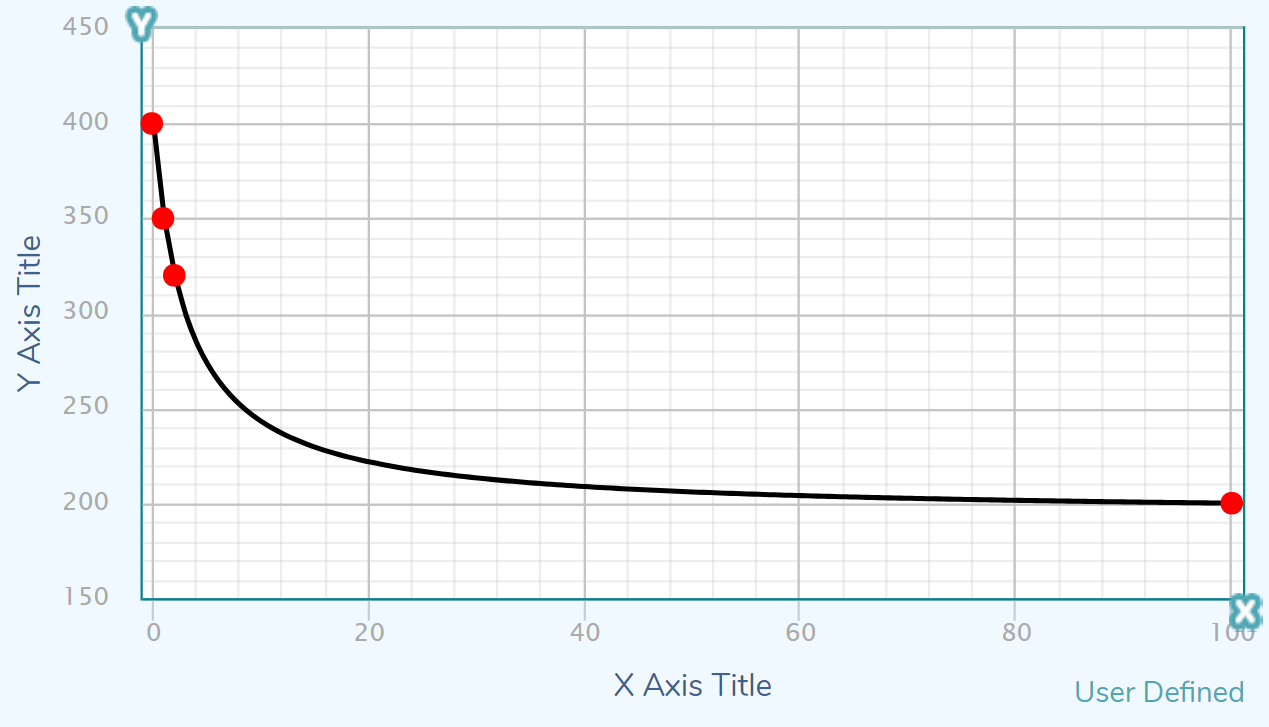
\includegraphics[width=0.48\textwidth, height=4cm]{curve-fit}
\\



\bibliographystyle{plainnat}
\bibliography{Biblio}

\end{multicols}
\end{document}